%% ##############################################################################################
%%
%% Copyright 2012 CNRS, INPT
%%  
%% This file is part of qr_mumps.
%%  
%% qr_mumps is free software: you can redistribute it and/or modify
%% it under the terms of the GNU Lesser General Public License as 
%% published by the Free Software Foundation, either version 3 of 
%% the License, or (at your option) any later version.
%%  
%% qr_mumps is distributed in the hope that it will be useful,
%% but WITHOUT ANY WARRANTY; without even the implied warranty of
%% MERCHANTABILITY or FITNESS FOR A PARTICULAR PURPOSE.  See the
%% GNU Lesser General Public License for more details.
%%  
%% You can find a copy of the GNU Lesser General Public License
%% in the qr_mumps/doc directory.
%%
%% ##############################################################################################

%% 
%% $Date: 2015-10-27 22:41:03 +0100 (mar., 27 oct. 2015) $
%% $Author: abuttari $
%% $Version: 1.1$
%% $Revision: 1980 $
%%

\begin{adjustwidth}{-0em}{-0em}
\thispagestyle{empty}


\vspace{10cm}
\vspace*{\stretch{1}}

{\noindent\hfill 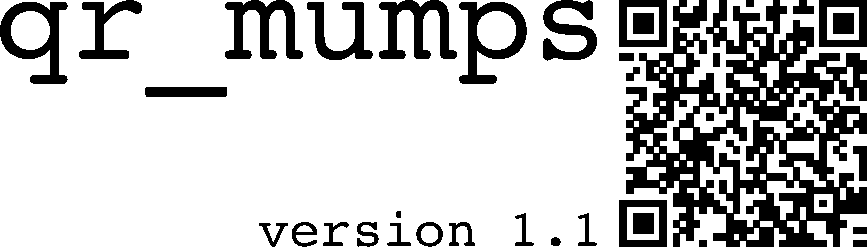
\includegraphics[width=0.9\linewidth]{figures/qrqr_cover.pdf}}

\noindent\rule{\linewidth}{5pt}\\[2.5ex]

\vspace{1cm}

\hspace{\stretch{1}}{\Large Users guide}
% \hspace{\stretch{1}}{\Large Alfredo Buttari}

% \hspace{\stretch{1}}{\large CNRS-IRIT}

% \hspace{\stretch{1}}{\large 19/01/2012}

\vspace*{\stretch{2}}

\end{adjustwidth}
%%% Local Variables: 
%%% mode: latex
%%% TeX-master: "qrm_ug"
%%% End: 
